\chapter{Backend}

Bevor wir zur Besprechung der Umsetzung des eigentlichen Backends übergehen, wollen wir zuerst einige grundsätzliche Überlegungen zur Art des Prozesses, den wir für unser Backend einsetzen wollen, festhalten.

\section{Art des Prozesses}\label{lbl_prozess_art}

\subsection{Prozesse unter Android}\label{lbl_be_procandroid}

Da in der Entwicklung für das Android-Betriebssystem ein etwas erweitertes Vokabular für die Beschreibung des Applikations-Lebenszyklus verwendet wird, wollen wir zuerst kurz auf einige dieser Begriffe im Android-Kontext eingehen.

Applikationen laufen unter Android grundsätzlich in einem eigenen Thread den das Betriebssystem als separaten Linux-Prozess startet und werden auch vom Betriebssystem wieder beendet. Sollen Komponenten in einem eigenen Prozess laufen, können weitere Threads gestartet werden\cite{adglc}. Diese können über die Standard Thread-Objekte von Java erzeugt werden, werden aber mit dem Applikations-Prozess terminiert, sollte Android entscheiden, dass dieser nicht mehr benötigt wird. Um dies, wenn Ressourcen benötigt werden sollten, möglich effizient durchzuführen, werden Prozesse vom Betriebssystem einfach abgewürgt (ein kill-Signal wird gesendet) und keinerlei Aufräumfunktionen werden ausgeführt. Applikationen sind daher selbst dafür verantwortlich, ihren Status zu sichern, wenn sie in den Hintergrund geschickt werden\cite{adbmt}.

Unser Erkennungs-Backend sollte nun aber auch unabhängig vom Frontend weiterlaufen. Grundsätzlich wäre das Beenden des Backend-Threads beim Schliessen des Frontends kein grösseres Problem, da wir davon ausgehen können, dass eventuell erst nach Beendung des Frontend-Threads eintreffende Resultate für den Benutzer nicht mehr relevant sind und verworfen werden können bzw. nicht mehr fertig gerechnet werden müssen. Allerdings wäre es zu bevorzugen, wenn bei einem erneuten Aufruf des Frontends der Backend-Thread schon im Speicher vorhanden ist und nicht noch neu initialisiert werden muss. Die Initialisierung des Backends kann je nach verwendeter Erkennungs-Methodik recht aufwendig sein. So muss etwa bei der Graphen-Methode zuerst die XML-Datei, in welcher der Graph gespeichert ist, eingelesen und der Graph aufgebaut werden. Der Benutzer erwartet möglichst schnell mit der Eingabe beginnen zu können und eine Initialisierung bei jeder Versuch dazu sollte ihm daher nicht zugemutet werden.

Neben den normalen Threads aus Java kennt Android noch spezialisierte Prozesse, die unabhängig von der Ursprungs-Applikation weiterlaufen können. Für uns interessant sind hier vor allem die Services und die Broadcast-Receiver.

\subsubsection{Broadcast-Receiver}

Broadcast-Receiver werden hauptsächlich dazu verwendet, im Hintergrund auf Ereignisse zu reagieren. Die Handhabung diese Ereignisses durch den Receiver muss innerhalb einer gegebenen Zeit erfolgen\footnote{Im Moment beträgt die zur Verfügung stehende Zeit 10 Sekunden, danach kann der Prozess jederzeit abgewürgt werden\cite{adbmt}}, wodurch diese nur im Speicher gehalten werden müssen, wenn ein solches Ereignis eintrifft. Broadcast-Receiver sind daher also gut geeignet um kurze Arbeiten als Reaktion auf eine externen Stimulus durchzuführen und werden etwa benutzt um auf Alarme oder Positions-Änderungen zu reagieren. Da sie aber nach Beendigung ihrer Aufgabe voraussichtlich wieder terminiert werden, würden sie für unseren Backend-Prozess keinen Vorteil darstellen, da sich die Frage der Reinitialisierung ebenfalls wieder stellen würde.

\subsubsection{Services}

Services sind unter Android sehr vielseitig und durch sie können Applikationen langlaufende Operationen im Hintergrund ausführen. Grundsätzlich ist ihre Laufzeit nicht beschränkt und ihr Verhalten in dieser Zeit wird weitestgehend von der Applikation bestimmt. So können sie etwa vom restlichen Programm unabhängige Operationen ausführen, auf gemeinsame Singleton-Objekte zugreifen oder gar in einen eigenen Prozess ausgelagert werden.

Services können allerdings vom Betriebssystem jederzeit abgeschossen werden, wenn es Ressourcen benötigen sollte. Allerdings wird sich Android merken, wenn es Services, die weiter laufen wollen, terminiert. Wenn wieder genug Arbeitsspeicher verfügbar ist, werden die beendeten Services wieder neu gestartet. Auch ist es möglich, dass Services beantragen, als Vordergrund-Prozesse behandelt zu werden und so recht gut vor dem Terminieren geschützt sind. Dies muss dem Benutzer allerdings angezeigt werden, damit sich dieser des laufenden Prozesses bewusst ist.

Für unser Backend sollte ein Service also die am besten geeignete Prozess-Form sein, da wir den Backend-Service im Hintergrund weiter laufen lassen können, nachdem eine Eingabe getätigt wurde. Eine Terminierung bei zu wenig vorhandenem Speicher können wir akzeptieren, da der Service danach wieder neu gestartet werden sollte und die Initialisierung vom Benutzer unbemerkt im Hintergrund stattfinden kann. Wir benötigen daher auch nicht die Privilegien eines Vordergrund-Prozesses.
%================================================

\section{Analyse}

\subsection{Initialisierung}

\subsection{Ablauf der Erkennungs}

Um den Ablauf der Erkennung möglichst flexibel zu machen, wurde dieser in mehrere Phasen aufgeteilt. Einige dieser Phasen sollen wiederum in mehrere Einzelschritte aufgeteilt werden.

\begin{figure}[h]
   \centering
   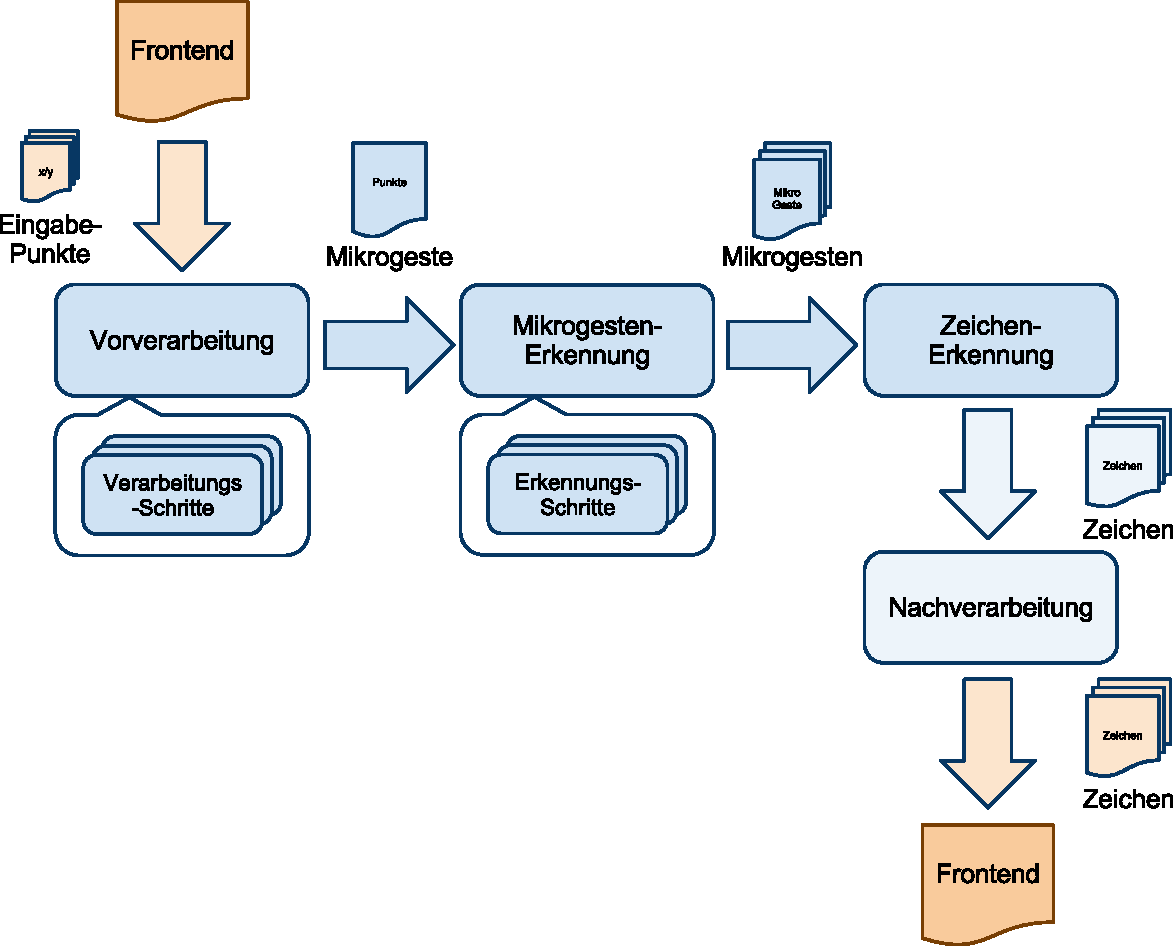
\includegraphics[width=\textwidth]{img/erkennungs_ablauf.pdf} 
   \caption{Erkennungs-Ablauf}
   \label{fig:erkennungs_ablauf}
\end{figure}

Zuerst soll eine Vorverarbeitung der Eingabe-Punkte durchgeführt werden, in der etwa eine Normierung, eine Glättung, eine Filterung oder ähnliches dieser durchgeführt werden kann. Diese Verarbeitungs-Schritte sollen sich nicht gegenseitig ausschliessen, sollen aber auch optional sein, da einige der dazu möglichen Algorithmen sehr rechenaufwendig sind.

Die zweite Phase soll die Erkennung der Mikrogesten sein. Auf diese soll in mehrere Erkennungs-Schritte aufgeteilt sein, die gegebenenfalls auch deaktiviert werden können.

Als nächstes soll die Zeichen-Erkennung durchgeführt werden. Diese soll allerdings in sich geschlossen funktionieren und nicht zwingend weiter in Teil-Schritte aufgeteilt werden. Das Erkennungs-Verfahren als ganzes soll allerdings austauschbar sein.

Die vierte und letzte Phase soll die Nachverarbeitung der erkannten Zeichen sein. Dies kann etwa bedeuten, das gewisse Zeichen wieder verworfen werden oder das die Gewichtung der Erkennungs-Wahrscheinlichkeit der Zeichen angepasst wird.

\subsubsection{Vorverarbeitung}

Häufig könnte die Erkennungsgenauigkeit der Mikrogesten-Erkennung durch eine passende Vorverarbeitung der Eingabe-Punkte erheblich verbessert werden. Allerdings sind viele der geeigneten Algorithmen sehr rechenaufwendig und können die Geschwindigkeit der Erkennung selbst auf leistungsfähigen Systemen erheblich verlangsamen\footnote{Unsere Test-Hardware, das Nexus One von Google mit einem 1 GHz Snapdragon Prozessor, benötigte bei einigen Algorithmen etwa mehrere Sekunden für die Glättung der Eingabe-Punkte normaler Buchstaben}. Daher war es unser Ziel, den Einsatz solche Vorverarbeitungs-Algorithmen zwar zu ermöglichen, diese allerdings optional zu machen. Insbesondere soll es möglich machen, dass diese in einer späteren Version auch aus dem Frontend heraus zu aktivieren oder deaktivieren.

Auch wollten wir eine serielle Abarbeitung von mehreren Vorverarbeitungs-Schritten möglich zu machen. Dabei muss es möglich sein, diese in einer festlegbaren Reihenfolge ausgeführt werden. So könnte zum Beispiel gewünscht werden, dass zuerst gewisse Punkte heraus gefiltert werden, bevor eine Glättung durchgeführt wird, um den Rechenaufwand für diese zu reduzieren.

\subsubsection{Mikrogesten-Erkennung}

Auch bei der Erkennung der Mikrogesten soll es möglich sein, diese in mehrere Schritte aufzuteilen und diese in einer definierbaren Reihenfolge durchzuführen. Dies kann etwa zum Testen verschiedener Ansätze nützlich sein, aber auch zum Feintuning eines speziellen Ansatzes. Ein Beispiel wäre hierbei, dass zuerst die harten Kanten im Pfad der Eingabe-Punkte detektiert werden und danach die einzelnen Mikrogesten in diesen Kanten gesucht werden.

Auch hier soll eine Anpassung zur Laufzeit durch das Frontend grundsätzlich möglich sein und von unserem Design unterstützt werden.

\subsubsection{Zeichen-Erkennung}

Auch das Austauschen des Algorithmus zur Zeichen-Erkennung zur Laufzeit soll grundsätzlich möglich sein. Allerdings soll es nur möglich sein, diesen als Ganzes auszutauschen. Eine Unterteilung in Teilschritte soll nicht von der Architektur her vorgeschrieben werden und eine Umorganisation dieser während der Laufzeit ist nicht angedacht, da wir die eigentliche Zeichen-Erkennung als monolithischen Vorgang gestalten wollen.

So können verschiedene Ansätze zur Zeichen-Erkennung anhand der Mikrogesten miteinander verglichen und alternative Erkennungs-Strategien angeboten werden. Neben dem in dieser Arbeit verwendeten Ansatz für eine Erkennung durch einen Graphen, ist etwa eine Erkennung über ein neuronales Netz eine naheliegende Möglichkeit.

Speziell für eine Erkennungs-Ansatz über ein neuronales Netz, aber auch für den Graphen-Ansatz, wäre eine Möglichkeit zur Anpassung der zur Erkennung verwendeten Datenbasis von Vorteil. Daher wollen wir auch eine Möglichkeit zur Nachverarbeitung der Daten bieten.

\subsubsection{Nachverarbeitung}

Für die Nachverarbeitung wollen wir einen zur Zeichen-Erkennung analogen Ansatz verwenden. Das heisst dass es möglich sein soll, den verwendete Algorithmus auszutauschen, eine Unterteilung in Teilschritte soll aber nicht gefordert werden. Im Gegensatz zur Zeichen-Erkennung soll die Nachverarbeitung aber optional sein.

Mögliche Einsatz-Zwecke für Nachverarbeitungs-Algorithmen wäre etwa, wie bereits erwähnt, die Anpassung der vorhandenen Datenbasis an den individuellen Benutzer in einem Trainingsmodus, die weitere Einschränkung oder Anpassung der Erkennungs-Wahrscheinlichkeiten der erkannten Zeichen, etwa anhand eines Wörterbuches.
%================================================

\section{Design}

\subsection{Schnittstellen}\label{lbl_be_intrf}

Wie bereits in \ref{lbl_prozess_art} besprochen, wollen wir für das Backend einen Service definieren. Damit dieser auch wirklich unabhängig (also in einem eigenen Prozess) vom Frontend läuft, soll dieser ein Remote-Service sein. Dies bedeutet, dass wir für die Kommunikation zwischen dem Frontend und dem Backend Schnittstellen definieren müssen, um die Inter-Prozess-Kommunikation abzuwickeln. Android stellt dafür eine eigenen Dialekt der Interface Definition Language bereit, der sich wenig überraschend ``Android Interface Definition Language'' (kurz AIDL) nennt.\\
\\
Die Schnittstellen, die wir benötigen werden, lassen sich in zwei Gruppen unterteilen: Die eigentliche Zeichen-Erkennung und die Verwaltung der Erkennungs-Algorithmen und deren Konfiguration.\\

\begin{lstlisting} [caption={AIDL-Definitionen der Service-Schnittstelle},label=intrf_detection]
interface IDetectionService {
  //...

  void addTouchPoints(
    in List<TouchPoint> points, boolean start_detection);
  //...
  void endSample();

  List<String> getAvailableStrategies();
  List<String> getActiveStrategies();
  void reinitializeStrategies(int type);
  List<StrategyArgument> getStrategyConfiguration(
    String strategy_name, int type);
  void setStrategyArgument(
    in StrategyArgument argument, int type);
  void broadcastArgument(in StrategyArgument argument);
}
\end{lstlisting}
\newpage
\begin{lstlisting} [caption={AIDL-Definitionen der R\"{u}ckruf-Schnittstelle},label=intrf_detection]
oneway interface IReturnResults {
  void recognisedCharacters(
    in List<Character> characters);
  //...
}
\end{lstlisting}

\subsubsection{Zeichen-Erkennung}

Die Schnittstellen für die Zeichen-Erkennung sind relativ simpel und direkt: Es müssen Eingabe-Punkte an das Backend gesendet werden und es müssen die erkannten Zeichen an das Frontend zurück gegeben werden. Da die Rückgabe der erkannten Zeichen nicht zwingend unmittelbar nach der Übertragung der Eingabe-Punkte erfolgen muss, wird sie über ein eigenes Rückruf-Interface abgehandelt.

Das Interface \emph{IDetectionService} definiert dafür unter anderem die Methoden \emph{addTouchPoints()}, mit welcher neue Eingabe-Punkte an den Erkennungs-Dienst übermittelt und die Erkennung falls gewünscht gestartet werden kann, sowie \emph{endSample()}, welche eine Eingabe abschliesst und die Erkennung started.

Für die Rückgabe definiert das Rückruf-Interface \emph{IReturnResults} unter anderem die Methode \emph{recognisedCharacters()}, mit welcher die erkannten Zeichen an das Frontend zurück gegeben werden.

\subsubsection{Verwaltung und Konfiguration der Erkennungs-Algorithmen}

Für die Verwaltung der Erkennungs-Algorithmen stellt das Interface \emph{IDetectionService} zum Einen Methoden für das Auslesen der verwendeten Algorithmen und zum Anderen für solche für die Konfiguration der einzelnen Algorithmen bereit.

Die Methode \emph{getAvailableStrategies()} gibt alle im Service vorhandenen Algorithmen zurück, während \emph{getActiveStrategies()} nur die momentan aktiven liefert. Ein solcher Algorithmus kann über die Konfigurations-Schnittstellen aktiviert oder deaktiviert werden. Weiter können mit der Methode \emph{reinitializeStrategies()} alle Algorithmen einer bestimmten Phase\footnote{Wird als Type der Phase ein Wert unter Null angegeben, werden alle Algorithmen neu initialisiert.} neu initialisiert werden werden.

\label{lbl_be_enable}Für die Konfiguration der Algorithmen wurde die Klasse \emph{StrategyArgument} entworfen, welche das Interface \emph{Parcelable} des Android-Frameworks implementiert und daher über die Kommunikations-Mechanismen von Android versandt werden kann. Die Klasse repräsentiert ein Argument eines Algorithmus und enthält dessen Namen, den Namen des Argumentes, sowie dessen Wert und Beschreibung. Ein Spezialfall eines solchen Arguments ist die Aktivierung oder Deaktivierung eines Algorithmus. Mit einem \emph{StrategyArgument} mit dem Namen ``enabled'' und dem Wert "false" kann ein Algorithmus deaktiviert werden, alle anderen Wert aktivieren ihn. Mit der Methode \emph{getStrategyConfiguration()} können alle Argumente eines Algorithmus ausgelesen werden. Die Methode \emph{setStrategyConfiguration()} setzt den Wert des übergebenen Arguments in dem im \emph{StrategyArgument} spezifizierten Algorithmus. Weiter ist auch noch die Methode \emph{broadcastArgument()} definiert, welche den Wert des übergebenen Argumentes in allen Algorithmen setzt, welche dieses unterstützen. Diese Methode wird etwa dafür verwendet, die Höhe des jeweiligen Eingabe-Feldes an alle interessierten Algorithmen zu melden.

\subsection{Erkennungs-Alogrithmen}

Da die einzelnen Schritte unseres Erkennungs-Ablaufs innerhalb der jeweiligen Phasen die selben Eingabe- und Ausgabe-Typen verwenden und dort austauschbar sein sollen lag die Anwendung des Strategy Design Patterns\cite[S.315-323]{designpatterns} für diese nahe. Jeder dieser Algorithmen ist somit eine Instanz einer der Phase entsprechenden Strategie.

Zur Verwaltung der Daten während der Erkennung benötigen wir drei Klassen: \emph{TouchPoint} für die Eingabe-Punkte, \emph{MicroGesture} für die Mikrogesten und \emph{Character} für die erkannten Zeichen. Die Mechanismen für die Interprozess-Kommunikation unter Android verschicken Objekte jeweils in einem so genannten \emph{Parcel}. Damit die genannten Klassen in ein solches verpackt ("marshaled") werden können, müssen sie das Interface \emph{Parcelable} implementieren. Diese definiert eine Methode, die das jeweilige Object in ein \emph{Parcel} packt.

Die Klasse \emph{TouchPoint} repräsentiert einen Punkt mit dessen Position, dem Zeitpunkt zu dem er eingegeben wurde und dessen Stärke (der Druck mit dem er eingegeben wurde)\footnote{Da die meisten modernen Android Mobiltelefone über kapazitive Touchscreens verfügen, welche Eingaben nicht anhand des Druckes erkennen, sondern über die Änderung eines elektrischen Feldes durch den Finger, wird die Stärke eines Punktes normalerweise den Wert "1.0" haben. Deshalb hat die Stärke für unsere Erkennung keinen Informationsgehalt und wird nicht beachtet.} und kann unter anderem die Entfernung zu einem anderen Punkt berechnen.

\begin{figure}[h!]
   \centering
   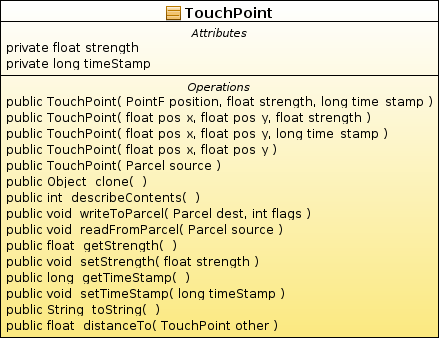
\includegraphics[scale=0.5]{img/uml_cd_tp} 
   \caption{Klassen-Diagramm \emph{TouchPoint}}
   \label{fig:cd_touchpoint}
\end{figure}

Die Mikrogesten in der Klasse \emph{MicroGesture} haben neben einer Liste mit den \emph{TouchPoints} aus welcher die Geste besteht auch einen Richtungs-Indikator und natürlich den Typ als welcher sie erkannt wurden als Attribute. Spezieller Methoden der Klasse sind etwa die Berechnung ihrer Gesamtlänge (jeweils von Punkt zu Punkt) oder das generieren eines Pfades aus den einzelnen Punkten.

\begin{figure}[h!]
   \centering
   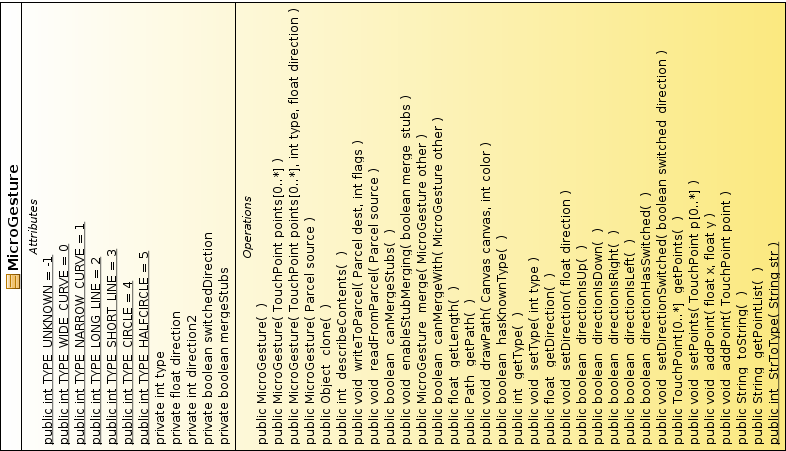
\includegraphics[width=\textwidth]{img/uml_cd_mg} 
   \caption{Klassen-Diagramm \emph{MicroGesture}}
   \label{fig:cd_microgesture}
\end{figure}

Die Klasse \emph{Character} umfasst neben dem erkannten Zeichen und dessen Erkennungs-Wahrscheinlichkeit optional auch die \emph{MicroGestures} aus denen das erkannte Zeichen besteht.

\begin{figure}[h!]
   \centering
   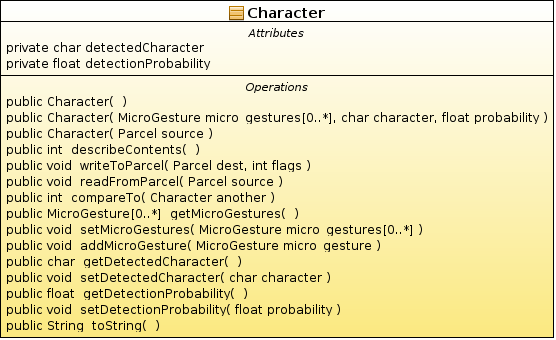
\includegraphics[scale=0.5]{img/uml_cd_char} 
   \caption{Klassen-Diagramm \emph{Character}}
   \label{fig:cd_character}
\end{figure}

\subsubsection{Strategien}

Da die Strategien aller Phasen ausser den Typen der Ein- und Rückgabewerte der Methode, die ihren eigentlichen Algorithmus implementiert, sehr ähnliche Attribute und Methoden haben, wurde ein globales Interface für die Strategien namens \emph{IStrategy} definiert, sowie eine abstrakte Basis-Klasse namens \emph{BaseStrategy} entworfen. Diese übernimmt etwa die Verwaltung der Argumente einer Strategie. Dadurch müssen die konkreten Implementationen von \emph{IStrategy}\footnote{Beziehungsweise der davon abgeleiteten Interfaces für die einzelnen Phasen.} nur den eigentlichen Algorithmus sowie ein paar einfache Methoden zur Beschreibung der Strategie umfassen. Dies erlaubt uns, Quelltext-Redundanzen zu minimieren und vereinfacht das Hinzufügen von neuen Algorithmen erheblich.

\subsubsection{Verwaltung der Strategien}

\begin{figure}[h!]
   \centering
   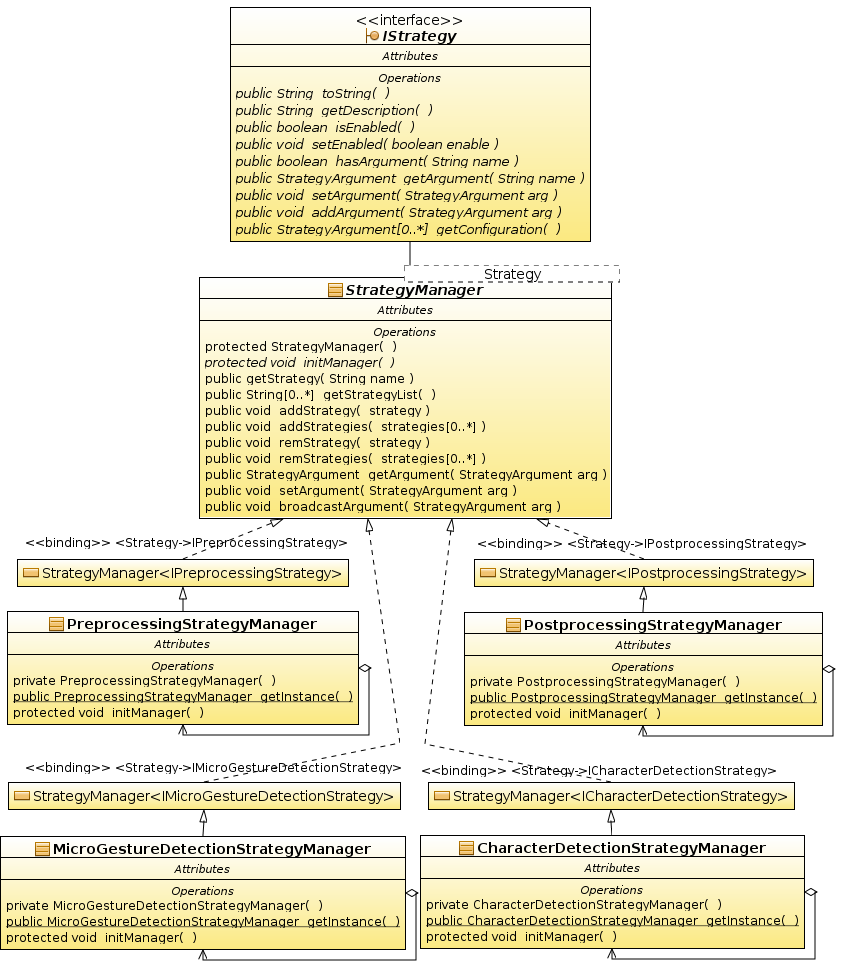
\includegraphics[width=\textwidth]{img/uml_cd_manager} 
   \caption{Klassen-Diagramm der Manager}
   \label{fig:cd_manager}
\end{figure}

Alle bekannten Strategien einer Phase werden zur einfachen Auffindbarkeit und Verwaltung durch entsprechenden Manager-Klassen verwaltet. Auf für die Manager der einzelnen Phasen wurde wieder eine verallgemeinerte abstrakte Basis-Klasse entworfen, welche die eigentlichen Verwaltungs-Operationen implementiert. Für die Implementation der Phasen-Manager wurden diese dann nur noch von der Basis-Klasse namens \emph{StrategyManager} abgeleitet und die einzelnen Strategien mussten noch initialisiert und dem Manager hinzugefügt werden (siehe Abbildung \ref{fig:cd_manager}). Die konkreten Manager-Klassen implementieren zusätzlich noch das Singleton Design Pattern\cite[S.127-134]{designpatterns}, damit die jeweiligen Strategietypen zentral von einem Objekte verwaltet und angesprochen werden können.

\subsection{Erkennungs-Service}\label{lbl_be_design_service}

Da der Erkennungs-Dienst als Service in einem unabhängigen Hintergrund-Prozess arbeiten soll, wird dieser natürlich von der Service-Klasse von Android abgeleitet und muss entsprechend die verlangten Methoden implementieren  (siehe Abbildung \ref{fig:cd_strategies} und Abschnitt \ref{lbl_be_impl_service} für die Implementation).

\begin{figure}[bh!]
   \centering
   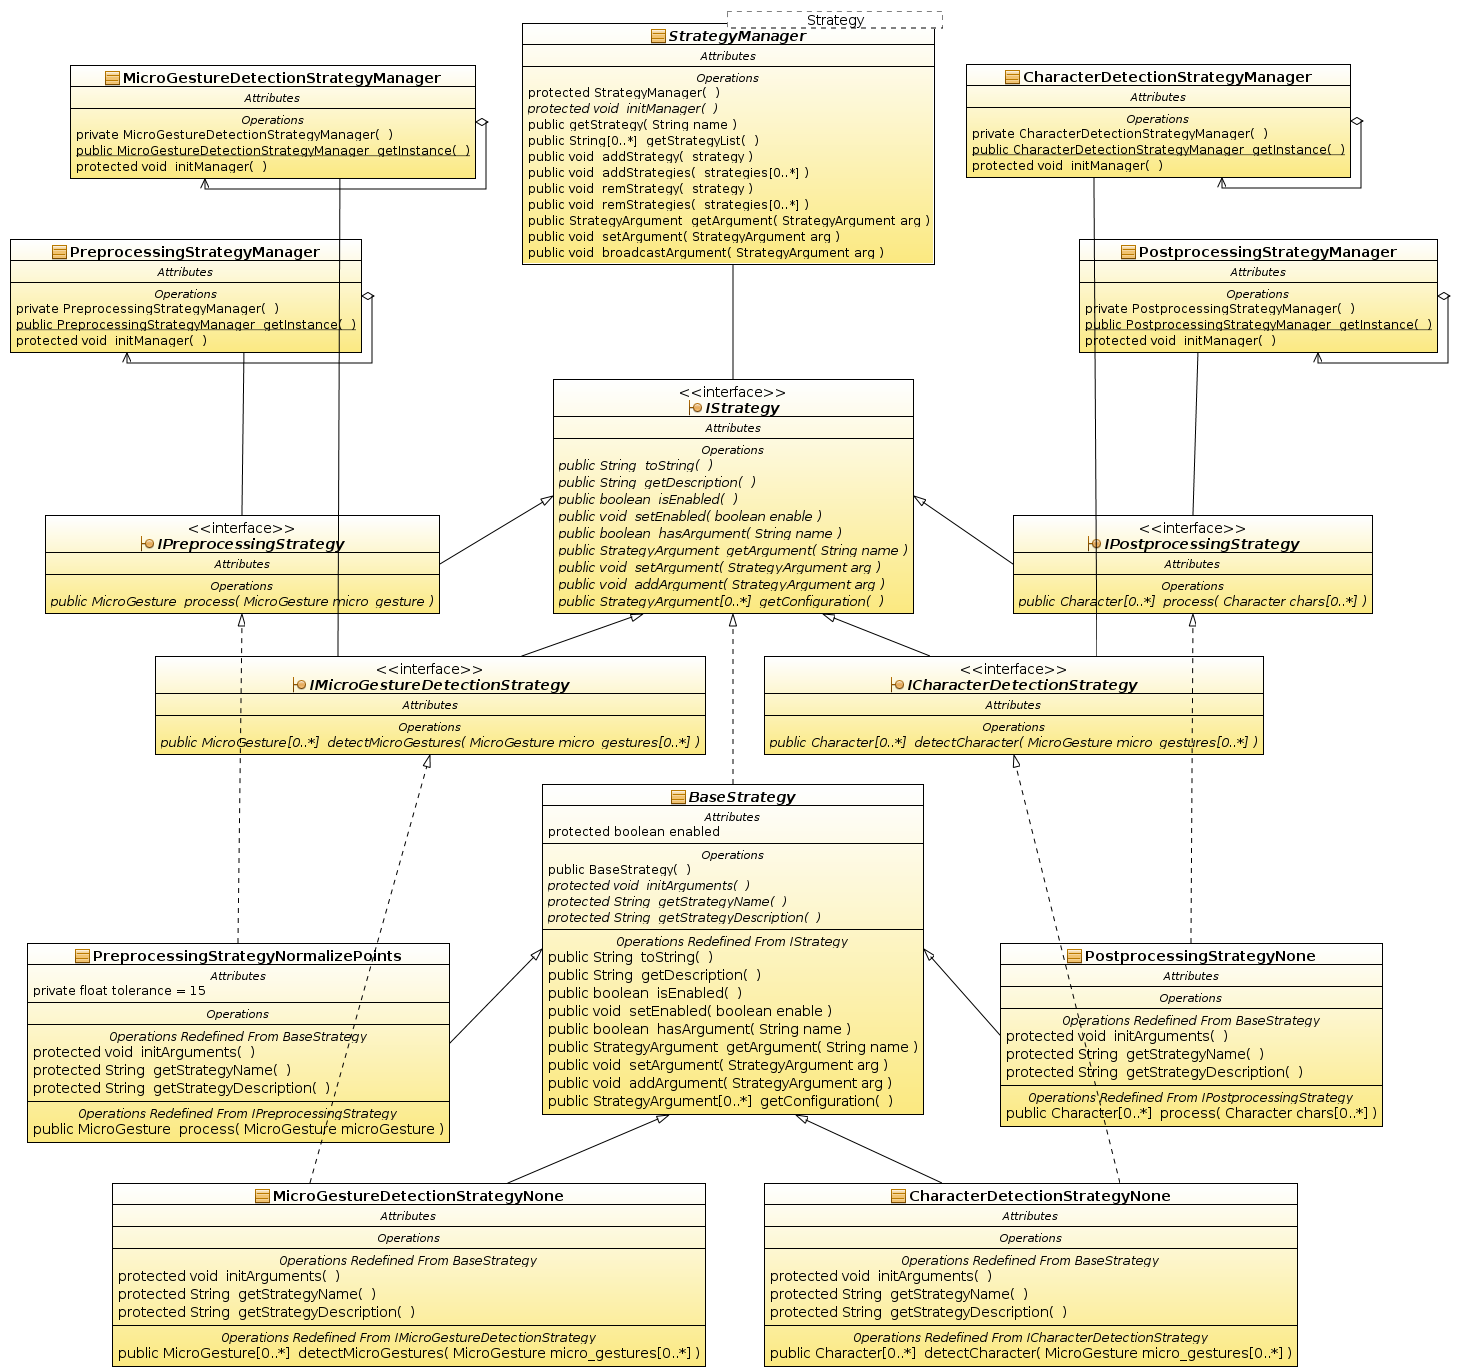
\includegraphics[width=\textwidth]{img/uml_cd_strategies} 
   \caption{Klassen-Diagramm der Strategien}
   \label{fig:cd_strategies}
\end{figure}

Weiter muss der Service den Ablauf seiner Erkennung verwalten. Dazu soll er für die beiden mehrstufigen Phasen jeweils eine Priority-Queue erhalten in welcher die einzelnen Erkennungs-Schritte anhand ihrer Position im Erkennungs-Prozess priorisiert abgelegt werden sollen (siehe Abbildung \ref{fig:cd_queues}).

\begin{figure}[bh!]
   \centering
   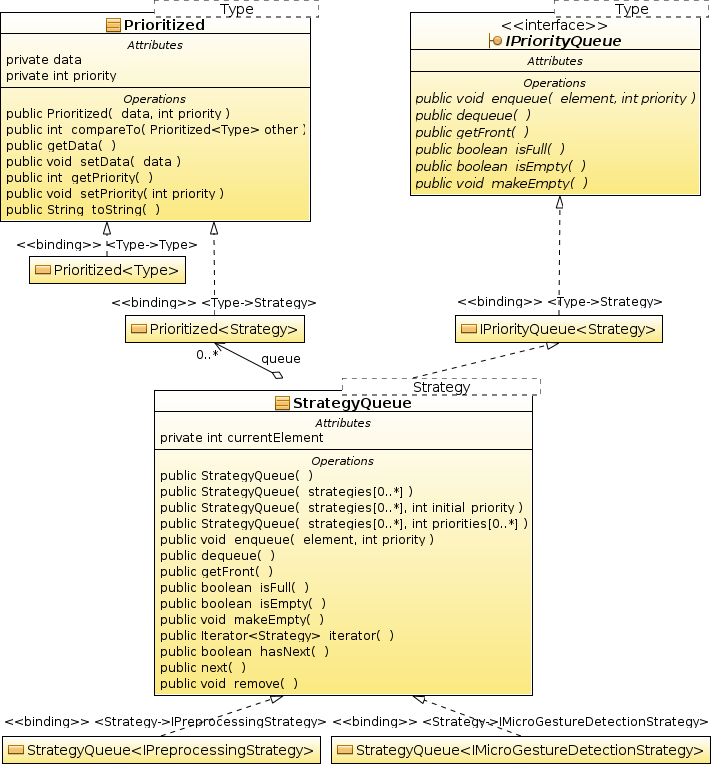
\includegraphics[width=\textwidth]{img/uml_cd_queue} 
   \caption{Klassen-Diagramm der Priority-Queues}
   \label{fig:cd_queues}
\end{figure}

Während der Erkennung muss der \emph{DetectionService} nun für jede Phase durch diese jeweilige \emph{StrategyQueue} iterieren und die aktiven Strategien, beziehungsweise bei einstufigen Phasen nur die entsprechende Strategie, anwenden. Zwischen den einzelnen Phasen muss der Dienst jeweils noch die Eingabe-Punkte oder die Resultate der vorgängigen Phase in das Eingabe-Format der nächsten Stufe konvertieren. Gegebenenfalls müssen vor dem Start der Erkennung noch die Eingabe-Punkte aus einem Buffer in die Liste der Eingabe-Punkte verschoben werden.

Nachdem alle Erkennungs-Phasen durchlaufen wurden, werden die Resultate dann über das Rückruf-Interface an alle angebunden Clients versendet (siehe Abbildung \ref{fig:sd_detection}).

\begin{figure}[bh!]
   \centering
   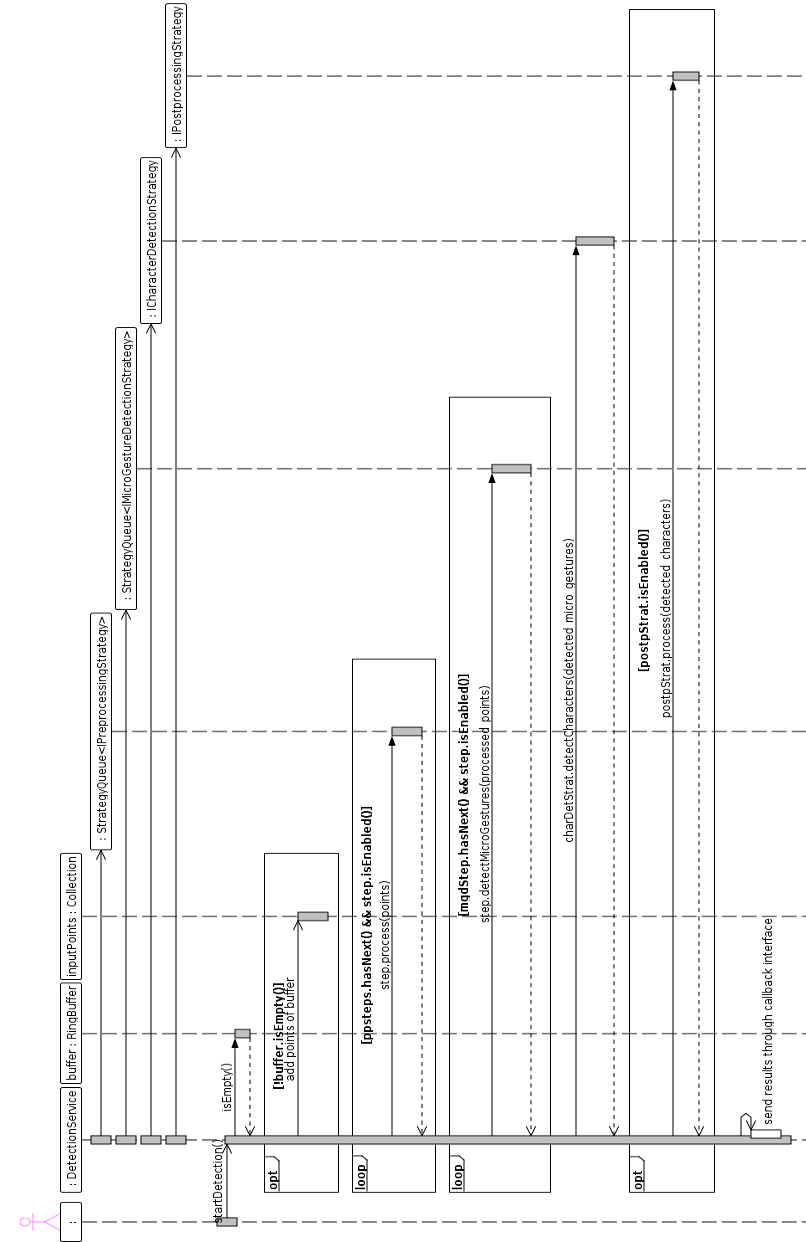
\includegraphics[scale=0.45]{img/uml_sd_detection} 
   \caption{Sequenz-Diagramm des groben Erkennungs-Ablaufs}
   \label{fig:sd_detection}
\end{figure}
%================================================

\section{Implementation}

In diesem Abschnitt sollen nur die interessanteren Aspekte der Implementation erläutert werden und die Erweiterung des Systems mit zusätzlichen Funktionen beschrieben werden. Für Details der Implementation soll hiermit auf die API-Dokumentation\footnote{Zu finden in Form von mit Javadoc und Doxygen generiertem HTML im Ordner ''doc'' unter dem Projektverzeichnis} und den Quellcode verwiesen werden.

\subsection{Strategien}

\subsubsection{Zeichen-Erkennungsstrategie Graph}

Um die Erkennung der Zeichen anhand der zuvor erkannten Mikrogesten mit Hilfe eines Graphen durchführen zu können, muss dieser zuvor initialisiert werden. Da wir uns eine gewisse Flexibilität bei der Definition des Graphen erhalten wollte, wurde entschieden, dessen Daten im standardisierten, XML-basierenden GraphML-Format\cite{graphml_primer} abzuspeichern und diese jeweils beim Start des \emph{DetectionService} einzulesen. Wie in \ref{lbl_be_procandroid} bereits erläutert, sollen die Daten des Graphen während der Laufzeit im Speicher gehalten werden, um die Verzögerung für den Anwender beim Aufstarten der Anwendung möglichst gering zu halten. Trotzdem soll es möglich sein, die mit der Applikation mitgelieferte GraphML-Datei durch eine eigene zu ersetzen, sollte der Benutzer dies wünschen oder ein Frontend dies umsetzen wollen.

Daher besitzt die Erkennungs-Strategie \emph{CharacterDetectionStrategyGraph} ein Argument das denn Ort an dem die GraphML-Datei gespeichert ist spezifizieren kann. Der Einfachheit halber wird neben dem Laden der mitgelieferten Datei aus den Applikations-Ressourcen nur das Laden von einer SD-Karte unterstützt. Der Benutzer oder ein Frontend müssten ihre eigene Datei daher auf eine solche ablegen. Damit können wir auch eventuelle Einschränkungen für den Dateizugriff umgehen\footnote{Unter Android laufen alle Applikationen mit einer individuellen Benutzer- und Prozess-Identifikation und das System erlaubt keinen Zugriff auf die Dateien anderer Applikationen.}.

Das eigentliche Laden des Graphen erfolgt in der \emph{initialize()} Methode der Strategie und verwendet das \emph{IGraphFactory} Interface. Dieses definiert eine Schnittstelle zur Erzeugung des Wurzel-Knoten eines Graphen nach dem Factory Method Design Pattern\cite[S.107-116]{designpatterns} und wird von der Klasse \emph{GraphFactoryGraphMLImport} implementiert. Diese delegiert das Erzeugen wiederum an das \emph{IGraphMLParser} Interface und dessen konkrete Implementation \emph{GraphMLPullParser}, welches einen XML Pull Parser\footnote{Im Prototyp wurde noch ein SAX-Parser verwendet, aber die Android API stellt zum Einlesen von XML-Dateien aus den Applikations-Ressourcen einen Pull Parser zur Verfügung, weshalb schlussendlich dieser verwendet wurde.} zum Einlesen der GraphML-Datei verwendet. \emph{GraphMLPullParser} versucht dabei zuerst, sofern der Parsing-Methode ein Pfad übergeben wurde, die entsprechende XML-Datei von der SD-Karte einzulesen. Ist diese nicht vorhanden, wird die im Applikations-Paket mitgelieferte GraphML-Datei eingelesen.

\begin{lstlisting} [caption={Initialisierung von \emph{CharacterDetectionStrategyGraph}},label=cds_graph_init]
public void initialize() {
  if (!hasArgument("Path")) {
    addArgument(new StrategyArgument(
      getStrategyName(), 
      "Path", "/sdcard/ba10_bsha_1.xml", 
      "Path of the GraphML file"));
  }

  IGraphFactory factory = new GraphFactoryGraphMLImport(
    getArgument("Path").getArgumentValue());
  root = factory.createRoot();	
}
\end{lstlisting}

Durch dieses Vorgehen muss der Graph nur beim ersten Aufstarten des Service geparsed und erzeugt werden und kann dann im Speicher gehalten werden. So lange ein Frontend an unseren \emph{DetectionService} gebunden ist, sollte dieser vom Betriebssystem nur im Falle eines äusserst gravierenden Ressourcen-Mangels terminiert werden. Da unser Frontend einen \emph{InputMethodService} implementieren wird und somit auch wenn der Benutzer keine Eingaben tätigt von Android im Hintergrund bereit gehalten wird, sollte dies beinahe nie der Fall sein. Sollte es trotzdem einmal erwünscht sein, den Graphen neu oder von einer anderen Datei einzulesen, kann über die Schnittstellen\footnote{Über die Methode \emph{reinitialize()} mit der Typen-Nummer der Zeichen-Erkennungsstrategie als Parameter. Soll eine andere Datei verwendet werden, muss diese zuerst mit über das entsprechende \emph{StrategyArgument} spezifiziert werden.} des \emph{DetectionService} eine Reinitialisierung der Zeichen-Erkennungs-Strategie veranlasst werden. Dabei wird auch der Graph neu aufgebaut.

\begin{figure}[h!]
   \centering
   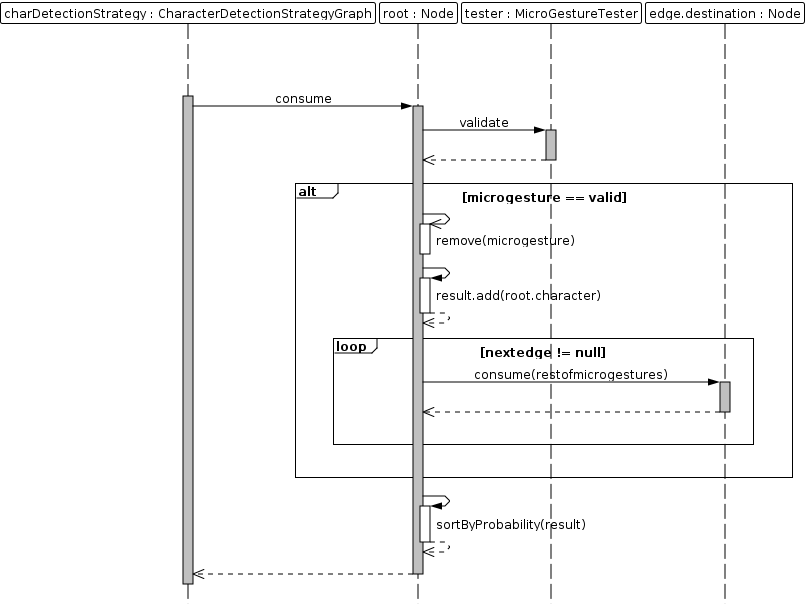
\includegraphics[width=\textwidth]{img/uml_sd_consume} 
   \caption{Sequenz-Diagramm des groben Erkennungs-Ablaufs in \emph{Node}}
   \label{fig:sd_consume}
\end{figure}

Werden dann später die erkannten Microgesten der Zeichen-Erkennung zugeführt, reicht die \emph{detectCharater()} Methode von \emph{CharacterDetectionStrategyGraph} diese an den Wurzel-Knoten des Graphen weiter. Dessen Methode \emph{consume()} nimmt diese entgegen, führt die Erkennung rekursiv durch und gibt die gefundenen Zeichen zurück.

Die Knoten tragen dabei den grössten Teil der zur Erkennung benötigten Informationen. Die Kanten nehmen die Gewichtung dieser Informationen vor, dienen ansonsten aber nur zum Verbinden der Knoten. Dadurch können diese Daten und deren Verarbeitung in die Klasse \emph{Node} konzentriert werden. 

Bei jedem Durchlauf von \emph{consume()} wird bei der Erkennung jeweils eine \emph{MicroGesture} vom aktuellen Knoten darauf getestet, ob sie sein Test-Kriterium erfüllt. Die Validierung des Kriteriums wird dabei an die Klasse \emph{MicroGestureTester} delegiert. Erfüllt die \emph{MicroGesture} das Kriterium, wird diese aus der Liste der zu konsumierenden \emph{MicroGestures} entfernt und das dem Knoten zugewiesene Zeichen wird, sofern vorhanden, der Liste der erkannten Zeichen angehängt. Danach werden die restlichen \emph{MicroGestures} den dem aktuellen Knoten im Graph folgenden Knoten zum Konsum zugeführt. Die jeweiligen Rekursions-Stufen geben dann jeweils die von ihnen erkannten Zeichen zurück, welche ebenfalls den Rückgabe-Zeichen der aktuellen Stufe angehängt werden.

Jede Rekursions-Stufe erhält auch ihre Erkennungs-Wahrscheinlichkeit übergeben, welche berechnet wird, indem die Wahrscheinlichkeit der übergeordneten Stufe mit dem Gewicht\footnote{Das Gewicht einer Kante im Graph repräsentiert die Wahrscheinlichkeit des Knotens zu dem die Kante führt.} der zur Stufe führenden Kante multipliziert wird. Die Erkennungs-Wahrscheinlichkeit wird jeweils mit dem erkannten Zeichen in der Klasse \emph{Character} zurückgegen. Die Liste der erkannten Zeichen wird dann vor der Rückgabe an die übergeordnete Stufe nach der Erkennungs-Wahrscheinlichkeit sortiert.
\newpage
\begin{lstlisting} [caption={Methode zur Zeichen-Erkennung in \emph{Node}},label=node_consume]
public Collection<Character> consume(
    Collection<MicroGesture> micro_gestures, 
    float probability) {
  ArrayList<Character> result;
  result = new ArrayList<Character>();
  //Weiterfahren wenn noch MicroGestures zum 
  //Konsum vorhanden sind
  if ((micro_gestures != null) 
      && (micro_gestures.size() > 0) 
      && (probability > MIN_PROBABILITY)) {
    //Testen, ob dem Node ein MicroGestureTester 
    //zugewiesen ist
    if (tester != null) {
      MicroGesture mg = micro_gestures.iterator().next();
      if (tester.validate(mg)) {
        //Positiv evaluierte MicroGestures aus den noch 
        //zu verfuetternden heraus nehmen
        micro_gestures.remove(mg);
        //Character des Nodes den Resultaten hinzufuegen
        result.add(new Character(
          null, character, probability));
        //Uebrige MicroGestures an die folgenden 
        //Knoten verfuettern
        for (Edge edge : outgoingEdges) {
          result.addAll(
            edge.getDestination().consume(
              micro_gestures, 
              (edge.getProbability() * probability)));
        }
      }
    //Alle MicroGestures an die folgenden Knoten ver-
    //fuettern wenn kein MicroGestureTester vorhanden
    } else {
      for (Edge edge : outgoingEdges) {
        result.addAll(
          edge.getDestination().consume(
            micro_gestures, 
            (edge.getProbability() * probability)));
      }
    }
  } //Resultate nach Wahrscheinlichkeit ordnen
  Collections.sort(result);
  return result;
}
\end{lstlisting}


\subsubsection{Beispiel einer neuen Strategie}

Zur Veranschaulichung wollen wir nun kurz demonstrieren, wie eine neue Strategie in unser System hinzugefügt werden könnte. Als Beispiel wollen wir jeweils eine Strategy implementieren, welche die übergebenen Eingabe-Punkte oder Mikrogesten, beziehungsweise die erkannten Zeichen über das Logcat Logging-Interface ausgibt und diese in eine Log-Datei schreibt. Diese könnten etwa als ersten und letzten Schritt der Vorverarbeitung eingebunden werden um deren Effekte zu beobachten, während die Mikrogesten-Erkennungsstrategie die erkannten Mikrogesten ausgeben würde und eine entsprechende Nachverarbeitungsstrategie die erkannten Zeichen. Die Implementation dieser Strategie-Typen erfolgt dabei nahezu identisch, da sich die Interfaces \emph{IPreprocessingStrategy}, \emph{IMircoGestureDetectionStrategy} und \emph{IPostprocessingStrategy} nur in den Typen ihre Parameter und Rückgabewerte unterscheiden. Daher soll hier nur die Implementation \emph{MicroGestureDetectionStrategyLog} explizit gezeigt werden.

Als erstes müssen wir dabei die abstrakten Methoden der Basis-Klasse \emph{BaseStrategy}, von der wir unsere Strategie ableiten, implementieren. Die beiden Beschreibungs-Methoden sind dabei ziemlich selbsterklärend. Sie geben den Namen beziehungsweise die Beschreibung der Strategie zurück. Die Methode \emph{initialize()} ist, wie ihr Namen vermuten lässt, dafür zuständig, die Strategie und ihre Attribute und Argumente zu initialisieren. In unserem Beispiel müssen wir ein Argument für den Pfad unserer Log-Datei festlegen\footnote{Falls die Strategie zu einem späteren Zeitpunkt neu initialisiert werden sollt, wird das Argument nur festgelegt, wenn es noch nicht vorhanden ist.}. Weiter soll die Log-Datei auch von einem Attribut vom Type \emph{File} repräsentiert und ein \emph{BufferdWriter} soll für das Schreiben in sie erzeugt werden.

\begin{lstlisting} [caption={Beispiel-Strategie \emph{MicroGestureDetectionStrategyLog}},label=mgdslog_init]
public class MicroGestureDetectionStrategyLog 
  extends BaseStrategy {

  private static final String TAG = "MGDS_Log";
  private File logFile;
  private BufferedWriter writer;

  public void initialize() {
    if (!hasArgument("Path")) {
      addArgument(new StrategyArgument(
        getStrategyName(), 
        "Path", "/sdcard/ba10_bsha_1.log", 
        "Path of the log-file"));
    }
    try {
      logFile = new File(
        getArgument("Path").getArgumentValue());
      if (!logFile.exists()) {
        logFile.createNewFile();
      }
      writer  = new BufferedWriter(
        new FileWriter(logFile, true));
    } catch (IOException ex) {
      Log.e(TAG, ex.getMessage(), ex);
    }
  }

  protected String getStrategyName() {
    return "Log";
  }

  protected String getStrategyDescription() {
    return "Logs the given MicroGestures " + 
           "into the specified log-file";
  }
}
\end{lstlisting}

Nun können wir uns daran machen, das Interface \emph{IMicroGestureDetectionStrategy} zu implementieren. Dieses definiert die Methode \emph{detectMicroGestures()}, welche wir nun implementieren werden. In ihr sollen alle übergebenen \emph{MicroGestures} über das Logcat-Interface ausgegeben und in die Log-Datei geschrieben werden und dann unverändert wieder zurück gegeben werden.

\begin{lstlisting} [caption={Beispiel-Strategie \emph{MicroGestureDetectionStrategyLog} - Implementation des Interfaces},label=mgdslog_interface]
public class MicroGestureDetectionStrategyLog 
  extends BaseStrategy 
  implements IMicroGestureDetectionStrategy {

  //...
  public Collection<MicroGesture> detectMicroGestures(
    Collection<MicroGesture> micro_gestures) {
    try {
      DateFormat format = new SimpleDateFormat(
        "dd.MM.yyyy HH:mm:ss");
      for (MicroGesture mg : micro_gestures) {
        //MicroGesture an Logcat senden
        Log.i(TAG, "MicroGesture: " + mg.toString());
        //MicroGesture in Log-Datei schreiben
        writer.append(format.format(new Date()));
        writer.append(": "); writer.append(TAG);
        writer.append(", detected MicroGesture: ");
        writer.append(mg.toString()); writer.append('\n');
      }
      writer.close();
    } catch (Exception ex) {
      Log.e(TAG, ex.getMessage(), ex);
    }
    return micro_gestures;
  }
}
\end{lstlisting}

Nun müssen wir die fertige Strategie noch dem entsprechenden Manager bekannt machen. Dies erfolgt im Falle unseres Beispiels in der Methode \emph{initManager()} Methode von \emph{MicroGestureDetectionStrategyManager}.

\begin{lstlisting} [caption={Beispiel-Strategie \emph{MicroGestureDetectionStrategyLog} - Manager},label=mgdslog_manager]
  protected void initManager() {
    addStrategy(new MicroGestureDetectionStrategyNone());
    //Erzeugen und Hinzufuegen der anderen Strategien...
    addStrategy(new MicroGestureDetectionStrategyLog());
  }
\end{lstlisting}

Schlussendlich muss die Strategie noch an der gewünschten Position der Priority-Queue für Mikrogesten-Erkennungs-Strategien hinzugefügt werden. Dies erfolgt in der \emph{initDetection()} Methode der Klasse \emph{DetectionService} (siehe Listing \ref{service_init}).

\subsection{Service}\label{lbl_be_impl_service}

Neben der eigentlichen Zeichen-Erkennung mussten für den Service natürlich noch diverse Methoden der Basis-Klasse \emph{Service} implementiert werden um den Lebenszyklus des Dienstes abzuhandeln und um die korrekte Kommunikation mir dem Frontend sicher zu stellen. Als Erstes wollen wir nun aber Erkennung als solches betrachten.

\begin{figure}[h!]
   \centering
   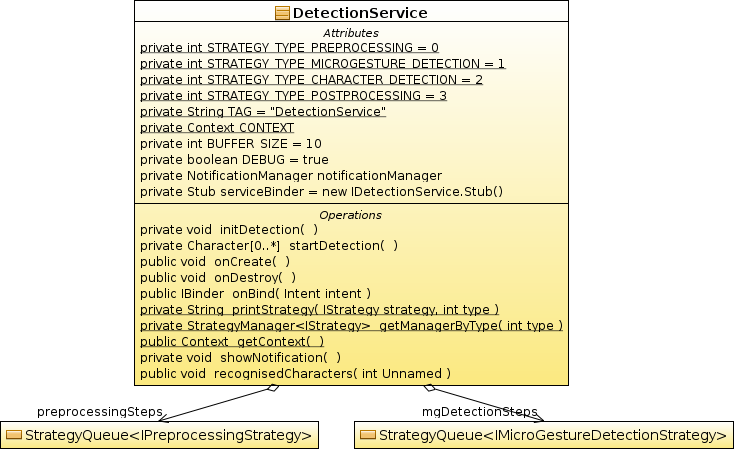
\includegraphics[width=\textwidth]{img/uml_cd_detectionservice} 
   \caption{Klassen-Diagramm des \emph{DetectionService}}
   \label{fig:cd_detectionservice}
\end{figure}

\subsubsection{Zeichen-Erkennung}

Neben einer Liste der Eingabe-Punkte, durch welche sich die Erkennung durcharbeiten soll, verfügt \emph{DetectionService} auch noch über eine Buffer, in dem Punkte abgelegt werden können. Die Erkennung kann entweder sofort starten, etwa wenn mehrere \emph{TouchPoints} zusammen übergeben wurden, oder sie kann automatisch starten, wenn der Buffer voll ist. Wird die Erkennung gestartet, werden die Punkte aus dem Buffer in die Liste der Eingabe-Punkte verschoben.

Die verwendeten Erkennungs-Algorithmen werden jeweils nach der gewünschten Reihenfolge geordnet in entsprechende \emph{StrategyQueues} abgelegt, oder bei einstufigen Phasen direkt als Attribut gesetzt. Diese Initialisierung erfolgt in der Methode \emph{initDetection()}.
\newpage
\begin{lstlisting} [caption={Initialisierung von \emph{DetectionService}},label=service_init]
  private void initDetection() {
    inputPoints = new ArrayList<TouchPoint>();
    buffer = new RingBuffer<TouchPoint>(BUFFER_SIZE);
    
    int priority = 1;
    preprocessingSteps = 
      new StrategyQueue<IPreprocessingStrategy>();
    preprocessingSteps.enqueue(
      PreprocessingStrategyManager.getInstance().
        getStrategy("NormalizePoints"), priority++);
    preprocessingSteps.enqueue(
      PreprocessingStrategyManager.getInstance().
        getStrategy("Spline"), priority++);	

    priority = 1;
    mgDetectionSteps = 
      new StrategyQueue<IMicroGestureDetectionStrategy>();
    mgDetectionSteps.enqueue(
      MicroGestureDetectionStrategyManager.getInstance().
        getStrategy("Edges"), priority++);
    //Hinzufuegen der anderen Strategien...
    mgDetectionSteps.enqueue(
      MicroGestureDetectionStrategyManager.getInstance().
        getStrategy("Log"), priority++);

    charDetectionStrategy = 
      CharacterDetectionStrategyManager.getInstance().
      getStrategy("Graph");
    postprocessingStrategy = 
      PostprocessingStrategyManager.getInstance().
      getStrategy("Log");
  }
\end{lstlisting}

Wird nun ein Durchlauf der Erkennung gestartet, läuft diese im Wesentlichen wie im Kapitel \ref{lbl_be_design_service} und dem dazugehörigen Sequenz-Diagramm (siehe Abbildung \ref{fig:sd_detection}) beschrieben ab. Zuerst werden eventuell im Buffer vorhandene Punkte in die \emph{inputPoints} verschoben. Die Eingabe-Punkte werden dann in einen temporären \emph{MicroGesture} Container kopiert und \emph{inputPoints} wird für den nächsten Durchlauf geleert.

Nun beginnt die Vorverarbeitungs-Phase, wo durch die Strategien der entsprechenden \emph{StrategyQueue} iteriert wird und die jeweilige \emph{IPreprocessingStrategy} wird, sofern sie aktiviert ist, auf die Punkte des temporären \emph{MicroGesture} Containers angewendet.

In der nächsten Phase, der Mikrogesten-Erkennung, erfogt nun ein Ablauf analog zu dem der Vorverabeitungs-Phase. Auch wird ein temporärer Container für alle erkannten \emph{MicroGestures} erzeugt und die zuvor bearbeitete \emph{MicroGesture} wird in diesen eingefügt. Darauf werden alle aktivierten Erkennungs-Schritte der \emph{StategyQueue} für die Mikrogesten-Erkennung mit dem Container durchlaufen.

Die nun folgende Zeichen-Erkennungs-Phase kann nun direkt den Container mit den erkannten \emph{MicroGestures} weiter verwenden. Da sie nur einstufig ist, können wir nun mit dem Container die in \emph{charDetectionStrategy} festgelegte \emph{ICharacterDetectionStrategy} durchlaufen und die erhalten erkannten Zeichen in unseren Rückgabewert speichern.

Als Letztes wird dann die Nachverarbeitungs-Phase durchlaufen, wobei die festgelegte \emph{IPostprocessingStrategy} direkt auf die erkannten Zeichen angewendet werden kann, falls diese aktiviert ist.

Da wir nun die eigentliche Erkennung abgeschlossen haben, müssen wir nun noch die Resultate an das Frontend zurück geben. Dazu wird ein Broadcast der Resultate an alle registrierten Clients über die in Kapitel \ref{lbl_be_intrf} beschriebene Rückruf-Schnittstelle \emph{IReturnResults} vorgenommen (siehe Listing \ref{intrf_detection} für die Schnittstellen-Definition unf Listing \ref{service_results} für deren Anwedung).

\begin{lstlisting} [caption={R\"{u}ckgabe der Resultate in \emph{DetectionService}},label=service_results]
    //...
    int i = callbacks.beginBroadcast();
    while (i > 0) {
      i--;
      try {
        callbacks.getBroadcastItem(i).
          recognisedCharacters(
            new ArrayList<Character>(result));
      } catch (RemoteException e) {}
    }
    callbacks.finishBroadcast();
    return result;
  }
\end{lstlisting}

\subsubsection{Service-Lebenszyklus und -Kommunikation}

Neben den zum Konstruktor beziehungsweise Dekonstruktor äquivalenten Methoden zum Service-Lebenszyklus \emph{onCreate()} und \emph{onDestroy()}\footnote{Welche neben der Initialisation der Erkennung nur noch für das Anzeigen einer \emph{Notification} über das Benachrichtigungs-System von Android während der Laufzeit des Service zuständig sind} müssen wir auch noch die Methode \emph{onBind()} implementieren. Diese gibt dem aufrufenden Client einen Stub\footnote{Ein Stub ist ein lokaler Anknüpfungspunkt um eine auf einem entfernten System erreichbare Komponente einfach anzusprechen.} unserer Kommunikations-Schnittstelle zum Service zurück, der noch implementiert werden musste (siehe Listing \ref{service_stub}). Über diesen Stub wird festgelegt, welche Operationen beim Aufruf der Schnittstellen-Methoden durchgeführt werden.

Neben der genannten Funktionalität umfasst die Klasse \emph{DetectionService} noch ein paar Helfer-Methoden, überwiegend für den \emph{IDetectionService}-Stub.

\begin{lstlisting} [caption={Implementation des \emph{IDetectionService} Interface-Stub},label=service_stub]
  private final IDetectionService.Stub serviceBinder = 
    new IDetectionService.Stub() {

    public void registerCallback(IReturnResults cb) 
      throws RemoteException {
      if (cb != null) {callbacks.register(cb);}
    }

    public void unregisterCallback(IReturnResults cb) 
      throws RemoteException {
      if (cb != null) {callbacks.unregister(cb);}
    }

    public void addTouchPoints(
      List<TouchPoint> points, boolean start_detection) 
      throws RemoteException {
      if (points != null) {
        inputPoints.addAll(points);
        if (start_detection || buffer.isFull()) {
          startDetection();
        }
      }
    }

    public void addTouchPoint(
      float pos_x, float pos_y, 
      float strength, long timestamp) 
      throws RemoteException {
      //...
    }

    public void endSample() throws RemoteException {
      startDetection();
    }

    public List<String> getAvailableStrategies() 
      throws RemoteException {
      //...
    }
    public List<String> getActiveStrategies() 
      throws RemoteException {
      //...
    }
    public void reinitializeStrategies(int type) {
      //...
    }
    public List<StrategyArgument> 
      getStrategyConfiguration(
        String strategy_name, int type) 
      throws RemoteException {
      //...
    }
    public void broadcastArgument(
      StrategyArgument argument) 
      throws RemoteException {
      //...
    }
    public void setStrategyArgument(
      StrategyArgument argument, int type) 
      throws RemoteException {
      //...
    }
  };
\end{lstlisting}
%================================================

